\documentclass{../tuda-exercise}

% Title information
\version{20. November 2021}
\sheetnumber{2}

\begin{document}

  \maketitle

  \begin{task}[credit=\stars{0}{3}]{Referenzen}
    Geben Sie in eigenen Worten wieder, was man unter einer Referenz versteht.

    \br

    Betrachten Sie außerdem folgendes Schaubild und den Codeausschnitt aus der Vorlesung:

    \begin{minipage}{0.45\textwidth}
      \begin{figure}[H]
        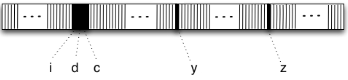
\includegraphics[width=1\textwidth]{graphics/V1_Task.png}
      \end{figure}
    \end{minipage}
    \hfill
    \begin{minipage}{0.45\textwidth}
      \lstinputlisting[style=Java]{codes/V1_01_Task.java}
    \end{minipage}

    Zeichnen Sie die Referenzpfeile nach den folgenden Aufrufen ein (ergänzen Sie auch die neuen
    Reservierungen des Speicherplatzes, wenn nötig):

    \lstinputlisting[style=Java]{codes/V1_02_Task.java}

    \begin{solution}
      Eine Referenz ist ein Zeiger auf eine Speicheradresse, an der ein Objekt gespeichert ist.
      \newpage
      Im folgenden sieht man die eingezeichneten Referenzpfeile:
      \begin{figure}[h]
        \centering
        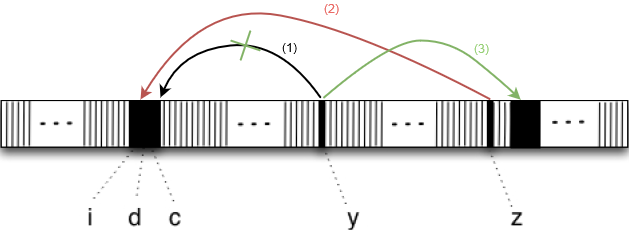
\includegraphics[width=0.8\textwidth]{graphics/V1_Solution.png}
      \end{figure}
    \end{solution}
  \end{task}


  \begin{task}[credit=\stars{0}{3}]{Zuweisen und Kopieren}
    Erläutern Sie in Ihren eigenen Worten den Unterschied zwischen Zuweisen und Kopieren. In
    welchen Fällen sind beide Aktionen synonym zu betrachten?

    \br

    Wie können Sie eine Zuweisung beziehungsweise eine Kopie in Java umsetzen? Nennen Sie jeweils
    ein Beispiel.

    \begin{solution}
      \begin{table}[h]
        \centering
        \begin{tabular}{p{22.5em}p{22.5em}}
          \toprule
          \textbf{Zuweisen} & \textbf{Kopieren}
          \\
          \midrule
          Zuweisungen werden mit dem Zuweisungsoperator \grqq =\grqq{} durchgeführt. Bei
          Referenztypen, also nicht primitiven Datentypen, wird die Adresse des Objekts
          zugewiesen, d.h. wenn wir zwei Objekte \inlinejava{a} und \inlinejava{b} vom Typ Object
          haben und \inlinejava{a = b} zuweisen, dann wird die Adresse des Objekts von
          \inlinejava{b} in \inlinejava{a} gespeichert. Beim Zuweisen wird also die Referenz auf
          dasselbe Objekt gesetzt.
          & Beim Kopieren eines Objekts wird jedes Attribut des Objekts in ein neues Objekt
          kopiert, sodass ein wertgleiches Objekt entsteht. Das neue Objekt weist aber nicht mehr
          Objektgleichheit zu dem anderen Objekt auf wie beim Zuweisen. Also beim Kopieren bleibt
          es bei zwei verschiedenen Objekten, aber ihre Attribute haben identische Werte.
          \\
          \bottomrule
        \end{tabular}
      \end{table}

      \br

      Synonym zu betrachten ist Zuweisen und Kopieren bei primitiven Datentypen, da es keine
      Aufteilung in Referenz und Objekt gibt. Durch die Zuweisung wird der tatsächliche Wert von
      primitiven Datentypen selbst in den neuen Speicherplatz kopiert.

      \begin{note}[title=Information:]
        Ein primitiver Typ ist von der Sprache vordefiniert und wird durch ein reserviertes
        Schlüsselwort gekennzeichnet. Sie können jeweils nur einen Wert speichern und, wie
        erwähnt, ist Zuweisung und Kopieren bei
        ihnen Synonym.

        \br

        Im Vergleich dazu speichert ein Referenztyp die Adresse des Objektes und nicht den im
        Objekt gespeicherten Wert.

        \br

        \lstinputlisting[style=Java]{codes/V2_Information.java}


        \begin{figure}[H]
          \centering
          \begin{memory}
            \allocatedummy{5}
            \allocatedummy{15}
            \allocatedummy{25}
            \allocate{7}{8}
            \allocate{20}{20}
            \assign{5}{7}{maxSpeed}
            \assign{10}{8}{fuel}
            \assign{20}{20}{car}
            \assignblock{20}{7}
          \end{memory}
          \caption{Abstrakte Visualisierung des Speicherplatzes eines Car-Objekts -
          \inlinejava{Car car = new Car();}}
          \label{fig:V2_Information}
        \end{figure}

        In der Abbildung \ref{fig:V2_Information} kann man sehen, dass die primitiven Datentypen
        \inlinejava{maxSpeed} und \inlinejava{fuel} direkt zugewiesen werden und \inlinejava{car}
        hingegen auf die Speicheradresse des Objekts referenziert.

        \br

        Mehr Informationen zu primitiven Datentypen finden Sie unter folgendem Verweis:

        \begin{center}
          \url{https://docs.oracle.com/javase/tutorial/java/nutsandbolts/datatypes.html}
        \end{center}
      \end{note}
    \end{solution}
  \end{task}

  \clearpage

  \begin{task}[credit=\stars{1}{3}]{Arrays}
    Welche Aussagen zu einem gegebenen Array \inlinejava{a} sind wahr?

    \begin{enumerate}
      [label=(\arabic*)]
      \item Alle Einträge des Arrays müssen vom selben Typ sein.
      \item Ein Array hat keine feste Größe und es können beliebig viele neue Einträge einem
      Array hinzugefügt werden.
      \item Um die Anfangsadresse einer Komponente an Index \inlinejava{i} zu bekommen, wird
      \inlinejava{i}-mal die Größe einer Komponente auf die Anfangsadresse von \inlinejava{a}
      addiert.
      \item Außer den eigentlichen Komponenten des Arrays enthält das Arrayobjekt nichts weiteres.
      \item Ein Array kann nur primitive Datentypen wie zum Beispiel \inlinejava{int},
      \inlinejava{char} oder \inlinejava{double} speichern. Somit ist es insbesondere nicht
      möglich, Roboterobjekte in einem Array zu speichern.
    \end{enumerate}

    Schreiben Sie die nötigen Codezeilen (auf Papier), um ein Array \inlinejava{a} der Größe
    \inlinejava{42} vom Typ \inlinejava{int} anzulegen. Füllen Sie danach das Array mithilfe
    einer Schleife, sodass an der Stelle \inlinejava{a[i]} der Wert \inlinejava{2i + 1} steht.
    Nutzen Sie dabei zuerst eine \inlinejava{while}- und danach eine \inlinejava{for}-Schleife.

    \begin{solution}
      \begin{enumerate}
        [label=(\arabic*)]
        \item Inkorrekt, denn ein Array kann auch Subtypen des eigentlichen Typs enthalten.
        \begin{itemize}
          \item Beispielarray von Typ \inlinejava{Number} und die davon abgeleiteten Klassen
          \inlinejava{Integer} und \inlinejava{Double}.

          \lstinputlisting[style=Java]{codes/V3_01_Solution.java}
        \end{itemize}
        \item Inkorrekt, denn ein Array ist statisch, d.h. es hat eine feste Größe.
        \item Wahr. Ein Array repräsentiert einen festen Block von reservierten Speicher eines
        gleichen Komponententyps (Datentyp). Die Adresse im Speicher bezieht sich bei einem Array
        auf die Speicheradresse des ersten Elements (Basisadresse). Die nachfolgenden Elemente
        können von der Basisadresse addiert mit einem Offset angesprochen werden. Dieser Offset
        entspricht die Größe des Komponententyps. Bspw. um das dritte Element eines Arrays
        anzusprechen:

        \begin{center}
          Basisadresse + 2 \(\cdot\) Offset
        \end{center}

        Das erste Element befindet sich unter der Basisadresse und das zweite Element unter
        Basiadresse + Offset.

        \begin{figure}[h]
          \centering
          \begin{memory}
            \allocatedummy{5}
            \allocatedummy{15}
            \allocatedummy{25}
            \allocate{8}{12}
            \allocate{18}{18}
            \assign{23}{18}{a}
            \assign{2}{8}{a[0]}
            \assign{5}{9}{a[1]}
            \assign{8}{10}{a[2]}
            \assign{14}{11}{a[3]}
            \assign{16}{12}{a[4]}
            \assignblock{18}{8}
          \end{memory}
          \caption{Abstrakte Visualisierung des Speicherplatzes eines Arrays \inlinejava{a}}
        \end{figure}

        \clearpage

        \item Inkorrekt, denn es ist noch die Größe des Arrays (\inlinejava{length})
        abgespeichert, die man berücksichtigen muss.
        \begin{itemize}
          \item Beispiel:
          \lstinputlisting[style=Java]{codes/V3_02_Solution.java}
        \end{itemize}
        \item Inkorrekt, denn es können auch Referenztypen in einem Array gespeichert werden.
        \begin{itemize}
          \item Beispielarray von Typ \inlinejava{Robot}:
          \lstinputlisting[style=Java]{codes/V3_03_Solution.java}
        \end{itemize}
      \end{enumerate}
      Die Codezeilen:
      \lstinputlisting[style=Java]{codes/V3_04_Solution.java}

      \lstinputlisting[style=Java]{codes/V3_05_Solution.java}
    \end{solution}
  \end{task}

  \clearpagesolution

  \begin{task}[credit=\stars{1}{3}]{Wettrennen}
    Sie haben einen schnellen Roboter \inlinejava{rabbit} erstellt und wollen ihm nun noch ein
    langsames Gegenstück \inlinejava{turtle} bauen. Beide starten an einem gemeinsamen Punkt,
    schauen in die gleiche Richtung und besitzen die gleiche Anzahl an Coins. Sie wollen nun
    schauen, wer in \inlinejava{10} Runden mehr Strecke zurücklegen kann. Jeder der beiden
    Kontrahenten kommt pro Runde genau einen Schritt voran, der schnelle \inlinejava{rabbit} erhält
    jedoch in jeder zweiten Runde einen Extraschritt. Betrachten Sie den folgenden
    Codeausschnitt, der die Situation implementieren möchte:

    \lstinputlisting[style=Java]{codes/V4_Task.java}

    Führen Sie den Code einmal selbst in Eclipse aus und schauen Sie was passiert! Beheben Sie
    danach alle vorhandenen Fehler in der Implementierung, um die oben beschriebene Situation
    exakt umzusetzen.

    \begin{solution}
      Probleme:
      \begin{enumerate}
        \item \inlinejava{rabbit} und \inlinejava{turtle} verweisen auf dasselbe Objekt.
        \item Die \textcolor{keywordcolor}{if}-Anweisung ermöglicht es nur, dass der
        \inlinejava{rabbit} in der zweiten Runde einen weiteren Schritt ausführen kann statt in
        jeder zweiten Runde.
      \end{enumerate}
      \lstinputlisting[style=Java]{codes/V4_Solution.java}
    \end{solution}
  \end{task}

  \clearpagesolution

  \begin{task}[credit=\stars{1}{3}]{Roboter miteinander vergleichen}
    Schreiben Sie eine Methode \inlinejava{int robotsEqual(Robot a, Robot b)}. Diese bekommt zwei
    Roboter übergeben und soll \inlinejava{2} zurückgeben, wenn die Attribute \inlinejava{x},
    \inlinejava{y}, \inlinejava{direction} und \inlinejava{numberOfCoins} bei beiden Robotern die
    gleichen Werte haben. \inlinejava{1} soll zurückgegeben werden wenn sich beide Roboter nur
    auf demselben Feld befinden, andernfalls gibt die Methode \inlinejava{0} zurück.

    \begin{solution}
      \lstinputlisting[style=Java]{codes/V5_Solution.java}
    \end{solution}
  \end{task}

  \clearpage

  \begin{task}[credit=\stars{2}{3}]{Primitive Datentypen}
    Schreiben Sie eine Methode \inlinejava{char smallestPDT(long n)}. Diese bekommt eine ganze
    Zahl übergeben und soll den primitiven Datentyp zurückgeben, der den wenigsten Speicherplatz
    verbraucht, aber immer noch die übergebene Zahl speichern kann. Geben sie
    \code{\textcolor{stringcolor}{"'l"'}} für den Datentyp \inlinejava{long} zurück,
    \code{\textcolor{stringcolor}{"' i"'}} für \inlinejava{integer} usw.

    \br

    Schreiben Sie nun eine Methode \inlinejava{char[] smallestPDTs(long[] a)}. Diese bekommt ein
    Array von ganzen Zahlen übergeben und soll ein Array zurückgeben, dass die Methode
    \inlinejava{smallestPDT(long n)}, in der gleichen Reihenfolge wie in \inlinejava{a}, auf
    jede Zahl in \inlinejava{a} anwendet.

    \begin{solution}
      \lstinputlisting[style=Java]{codes/V6_Solution.java}

      \begin{note}[title=Information:]
        Mithilfe des folgenden Verweises finden Sie mehr Informationen zu primitiven Datentypen:

        \begin{center}
          \url{https://docs.oracle.com/javase/tutorial/java/nutsandbolts/datatypes.html}
        \end{center}
      \end{note}
    \end{solution}
  \end{task}

  \begin{task}[credit=\stars{2}{3}]{Aufsummieren}
    Schreiben Sie eine Methode \inlinejava{void sumUp(int[] a)}, die ein Array \inlinejava{a} von
    Typ\inlinejava{int} erhält.

    \br

    An Index \(i \in \{0, \dots, \text{a.length-i}\}\) in \inlinejava{a} soll nun der Wert
    \(\text{a}[0] + \dots + \text{a}[\text{i}]\) geschrieben werden. Dabei bezeichnen
    \(\text{a}[0] + \dots + \text{a}[\text{i}]\) die Werte in \inlinejava{a} unmittelbar vor dem
    Aufruf der Methode.

    \br

    Übergeben wir der Funktion das folgende Array \inlinejava{a} = \([3, 4, 1, 9, -5, 4]\), so
    wird das Array folgendermaßen modifiziert:

    \begin{align*}
      & \rightarrow [3, 3 + 4, 3 + 4 + 1, 3 + 4 + 1 + 9, 3 + 4 + 1 + 9 + (-5),
      3 + 4 + 1 + 9 + (-5) + 4]
      \\
      & \rightarrow [3, 7, 8, 17, 12, 16]
    \end{align*}

    \begin{solution}
      \lstinputlisting[style=Java]{codes/V7_Solution.java}

      \begin{note}[title=Information:]
        Alternativ kann man die Zuweisung und Addition in Zeile 8 auch folgendermaßen darstellen:

        \begin{lstlisting}[style=Java]
					a[i] = a[i] + a[i - 1];
        \end{lstlisting}
      \end{note}
    \end{solution}
  \end{task}

  \clearpage

  \begin{task}[credit=\stars{3}{3}]{Liste von Positionen}
    In dieser Aufgabe werden wir ein wenig kreativ und zeichnen die Initialen der FOP mit dem
    FOP-Bot. Dazu müssen wir zunächst sicherstellen, dass unser Roboter eine beliebige gegebene
    Position automatisiert ansteuern kann.

    \br

    Um uns die Arbeit zu vereinfachen, verwenden wir die Klasse \inlinejava{Point} der
    Java-Standardbibliothek, deren Instanzen Punkte im zweidimensionalen Raum repräsentieren. Ein
    \inlinejava{Point}-Objekt kann mittels des Konstruktors \inlinejava{Point(int x)},
    \inlinejava{int y)} erzeugt werden. Die Abfrage der Werte ist dann über die Objekt-Attribute
    \inlinejava{x} und \inlinejava{y} möglich.

    \begin{subtask*}{Setzen der Blickrichtung}
      Als Erstes soll die \inlinejava{public}-Methode \inlinejava{void setDirection(Robot robot,
        Direction direction)} implementiert werden: Diese bekommt ein \inlinejava{Robot}-Objekt
      sowie eine \inlinejava{Direction}-Konstante übergeben. Nach Aufruf der Methode soll der
      Roboter in die gewünschte Richtung blicken.

      \begin{solution}
        \lstinputlisting[style=Java]{codes/V8_1_Solution.java}
      \end{solution}
    \end{subtask*}

    \clearpagesolution

    \begin{subtask*}{Bewegen zu einer Position}
      Implementieren Sie nun die \inlinejava{public}-Methode \inlinejava{void moveToPoint(Robot
      robot, Point point)}: Mit dem Aufruf der Methode soll der gegebenen Roboter mittels der
      soeben von Ihnen implementierten Methoden \inlinejava{setDirection} und der Ihnen bereits
      bekannten Methode \inlinejava{move} an die gegebene Position bewegen werden. Sie können
      davon ausgehen, dass sich auf dem Weg zu dieser Position keine Hindernisse befinden.
      Dabei ist nicht wichtig, dass der Roboter den kürzesten Weg findet.

      \begin{solution}
        \lstinputlisting[style=Java]{codes/V8_2_Solution.java}
      \end{solution}
    \end{subtask*}

    \clearpagesolution

    \begin{subtask*}{Coin Patterns}
      Nun implementieren Sie die \inlinejava{public}-Methode \inlinejava{void putCoins(Robot
      robot, Point[] points)}: Der gegebene Roboter soll an jeder der im gegeben Array
      enthaltenen Position eine Münze ablegen, sich anschließend in die Mitte der Welt bewegen
      und nach oben blicken.

      \begin{figure}[h]
        \centering
        \begin{FOPBotWorld}{11}{5}
          \foreach \x/\y in {
              {0/0},
              {0/1},
              {0/2},
              {0/3},
              {0/4},
              {1/4},
              {2/4},
              {1/2},
              {2/2},
              {4/0},
              {4/1},
              {4/2},
              {4/3},
              {4/4},
              {5/4},
              {6/4},
              {6/3},
              {6/2},
              {6/1},
              {6/0},
              {5/0},
              {8/0},
              {8/1},
              {8/2},
              {8/3},
              {8/4},
              {9/4},
              {10/4},
              {10/3},
              {10/2},
              {9/2},
          }{
            \putcoin{\x}{\y}{1}
          }
          \path (5,2) pic {Trianglebot};
        \end{FOPBotWorld}
        \caption{Gewünschtes Ergebnis}
      \end{figure}

      \begin{note}[title=Verbindliche Anforderung:, color=tuda-orange]
        Die einzelnen Positionen des \code{Point}-Arrays müssen in einer einzigen
        \inlinejava{for}-Schleife abgelaufen werden. Die Objektmethode \code{putCoin} der Klasse
        \code{Robot} darf nur innerhalb dieser \inlinejava{for}-Schleife aufgerufen werden.
      \end{note}

      \begin{solution}
        \lstinputlisting[style=Java]{codes/V8_3_Solution.java}
      \end{solution}
    \end{subtask*}
  \end{task}
\end{document}
